\renewcommand{\theequation}{\theenumi}
\begin{enumerate}[label=\arabic*.,ref=\thesubsection.\theenumi]
\numberwithin{equation}{enumi}

\item general equation for the circle can be given as
\begin{align}
\vec{x}^T\vec{x} + 2\vec{O}^T\vec{x} +\norm{O}^2 - \vec{r}^2 &= 0
\end{align}
given equation of circle
\begin{align}
\vec{x}^T\vec{x} -25&= 0
\end{align} 
comparing bothe of equation we can find the value of r and value of  $\vec{O}$
\begin{align}
\vec{r}&= 4
\\
\vec{O} &= \myvec{0\\0}
\\
\vec{A}-\vec{O} &= \myvec{-2.5\\3.5}
\\
\norm{\vec{A} - \vec{O}} &= 18.5
\\ 18.5 &\textless \vec{r}
\end{align} 
Thus it is clear that the length of OA is shorter than that of r so point$\vec{A} $exist inside the circle.
\begin{figure}[!ht]
	\centering
	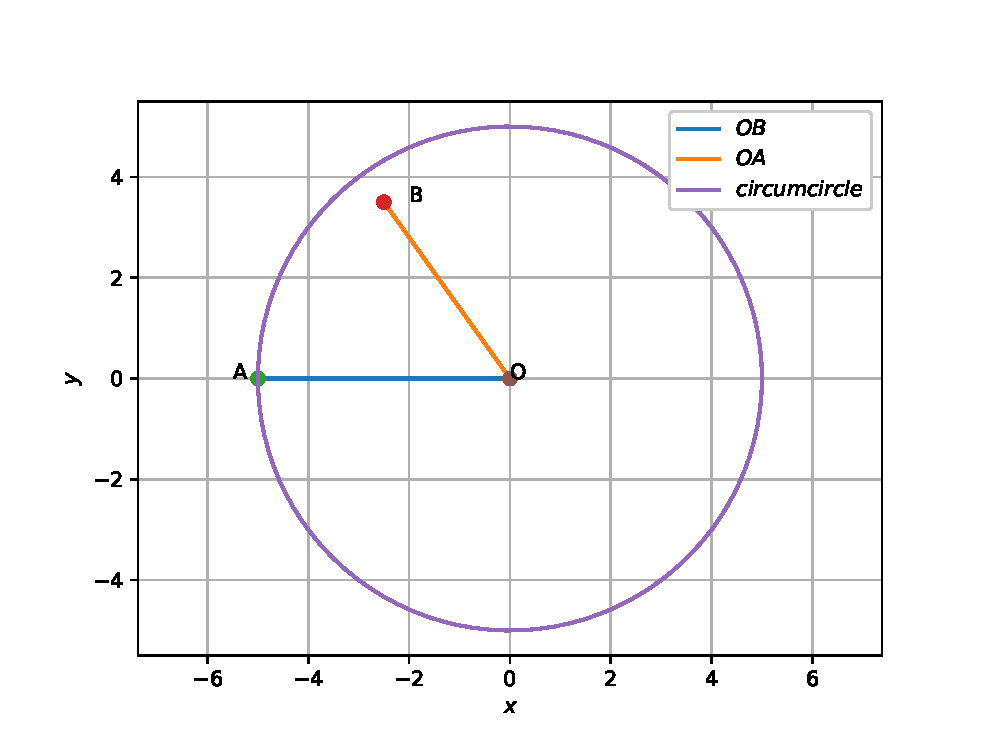
\includegraphics[width=\columnwidth]{./figures/circle/circle2.eps}
	\caption{circle }
	\label{fig:circle}
	path to the code for the above figure
	\begin{lstlisting}
	codes/circle/circle2.py
	\end{lstlisting}
\end{figure}
\end{enumerate}